\problem{}

SIST allows students to work as TAs but would like to avoid TA cycles. A TA cycle is a list of TAs ($A_{1}$, $A_{2}$, . . . , $A_{k}$) such that $A_{1}$ works as a TA for $A_{2}$ in some course, $A_{2}$ works as a TA for $A_{3}$ in some course, · · · , and finally $A_{k}$ works as a TA for $A_{1}$ in some course. We say a TA cycle is simple if it does not contain the same TA more than once. Given the TA arrangements of SIST, we want to find out whether there is a simple TA cycle containing at least K TAs. Prove this problem is NP-complete.

\solution{
To show that TA cycle problem is NP-complete, we should prove that the solution can be verified in polynomial time first. Assume that we have $k$ TAs, if we want to check whether they can be a TA cycle, one counts the vertices to make sure they are all there, then checks that each is connected to the next by an edge, and whether the last is connected to the first which takes time proportional to $O(k)$. $O(k)$ is a polynomial, so the check runs in polynomial time. In conclusion, the verification can be done in polynomial time and it's a NP problem.
	
Then we need a polynomial-time reduction from 3-SAT: Suppose there is variables set $U = \{x_1,..,x_n\}$, it's nagation is $\overline{U} = \{\neg x_1,..,\neg x_n\}$. $B = C_1\wedge...\wedge C_m$ is a boolean expression, where $C_i = (\alpha \vee \beta \vee \gamma),\alpha,\beta,\gamma \in U \cup \overline{U}$. 
\begin{itemize}
	\item For each variable $x_i\in U$, create vertices $c_{i,1},...,c_{i,3(m+1)}$, add $s,t$. Create edges $s\to c_{1,1},c_{1,3(m+1)}$; $c_{n,1},c_{n,3(m+1)}\to t$; for each $c_{i,j}\rightleftharpoons c_{i,j+1}$; $c_{i,1},c_{i,3(m+1)}\to c_{i+1,1},c_{i+1,3(m+1)}$.
	\item For each clause $C_i$, create a vertex. If $x_j$ appears in $C_i$ create edges $c_{j,3i}\rightleftharpoons C_i$ and $C_i \rightleftharpoons c_{j,3i+1}$. If $\neg x_i$ appears in $C_i$ create edges $c_{j,3i+1}\rightleftharpoons C_i$ and $C_i \rightleftharpoons c_{j,3i}$. 
\end{itemize}
\begin{figure}[ht]
	\centering
	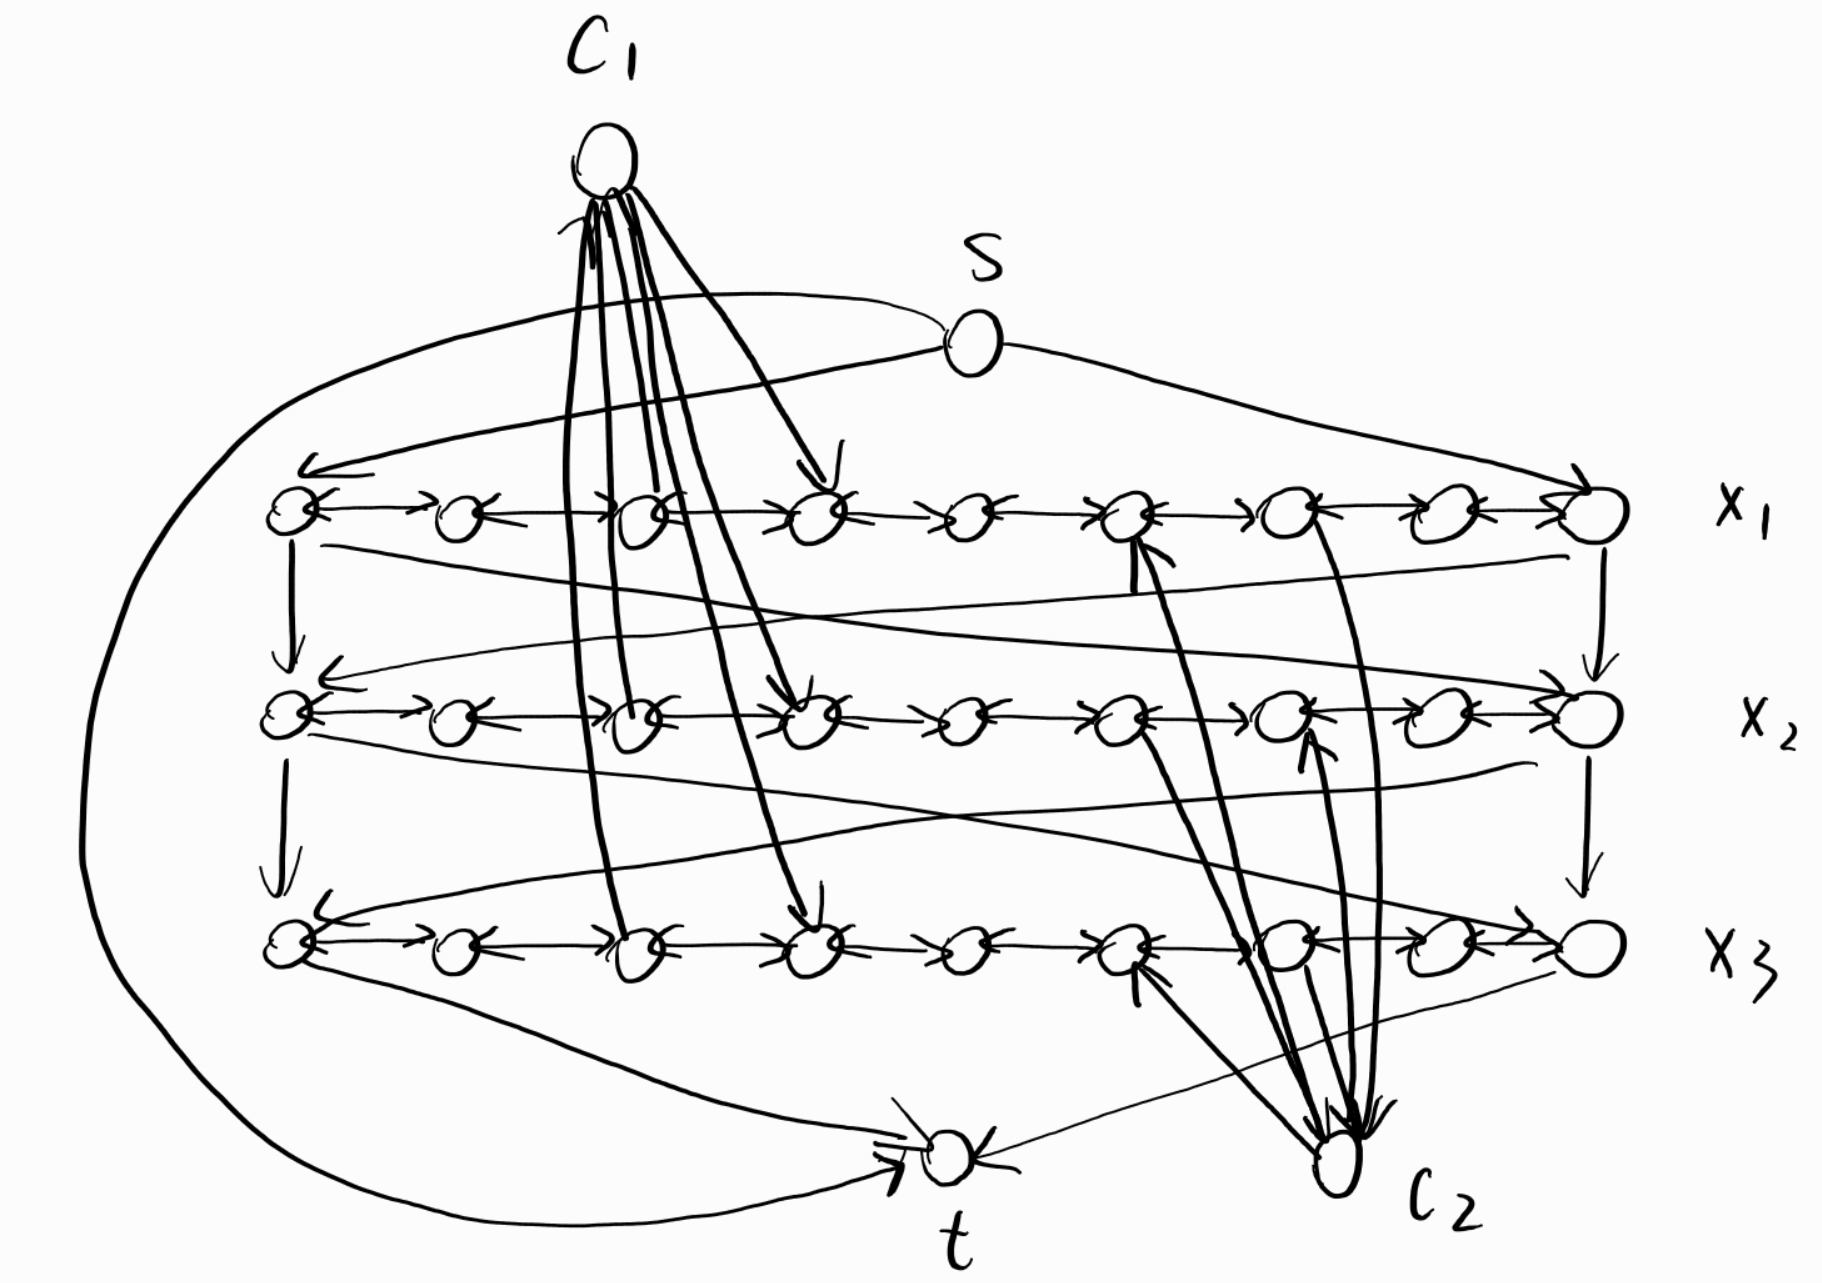
\includegraphics[scale=0.2]{q5.jpg}
	\caption{The graph from $B$.}
\end{figure}

It's easy to know that the graph contains $2+m+3(m+1)n$ vertices and $2mn+3m+5$ edges, which is constructed in polynomial time. Finally, we need to show yes-instances of 3-SAT map to yes-instances of TA cycle problem:

->: Suppose $T$ is a truth that satisfies $B$. Begin at $s$, go to $c_{1,1}$ or $c_{1,3(m+1)}$ for $x_1$ is true or false. Go along the row and may go through $C_i$ if it's available. Then go to $c_{2,1}$ or $c_{2,3(m+1)}$ if $x_2$ is true or false and continue. There will be at least one route to go through each $C_i$, and the path will visit every vertex of $G$. Therefore, we can find a TA cycle of $G$ when there is a satisfying truth assignment.

<-: Suppose $H$ is a TA cycle(Hamiltonian circuit) on $G$. It starts at $s$ and must go either $c_{1,1}$ or $c_{1,3(m+1)}$. Assume that $x_i$ is true if $H$ go to $c_{1,1}$ and false go to $c_{1,3(m+1)}$, continue to go through $x_2,..,x_n$, at last arrive $t$ to finish. It's known to us that each $C_i$ is traversed, which means each $C_i$ contains a $x_i$ or $\neg x_i$($x_i$ is boolean). Therefore, we can find a satisfying truth assignment when there is a TA cycle.

From the above aspects, it's proved that TA cycle problem is NP-complete.

}